\chapter{Metodologi}

Pada bab ini penulis menjelaskan mengenai metodologi yang digunakan selama pengerjaan tugas akhir.

\begin{figure}[H]
	\begin{centering}
		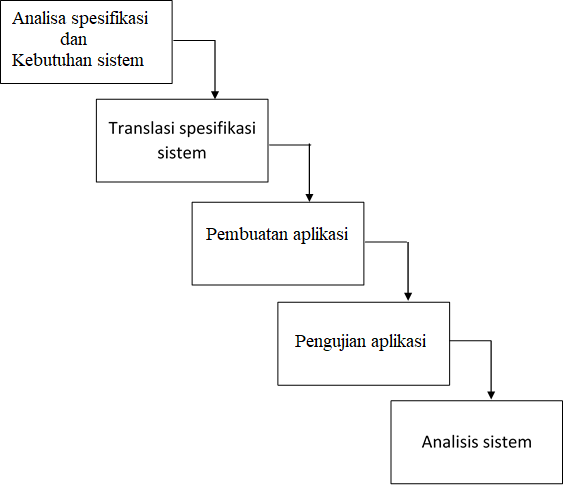
\includegraphics[scale=0.7]{metodologi_proposal}
		
		\caption{Metodologi.}
	\end{centering}
\end{figure}


\section{Alur Aplikasi}

Aplikasi akan memiliki diagram alir seperti berikut:

\begin{figure}[H]
	\begin{centering}
		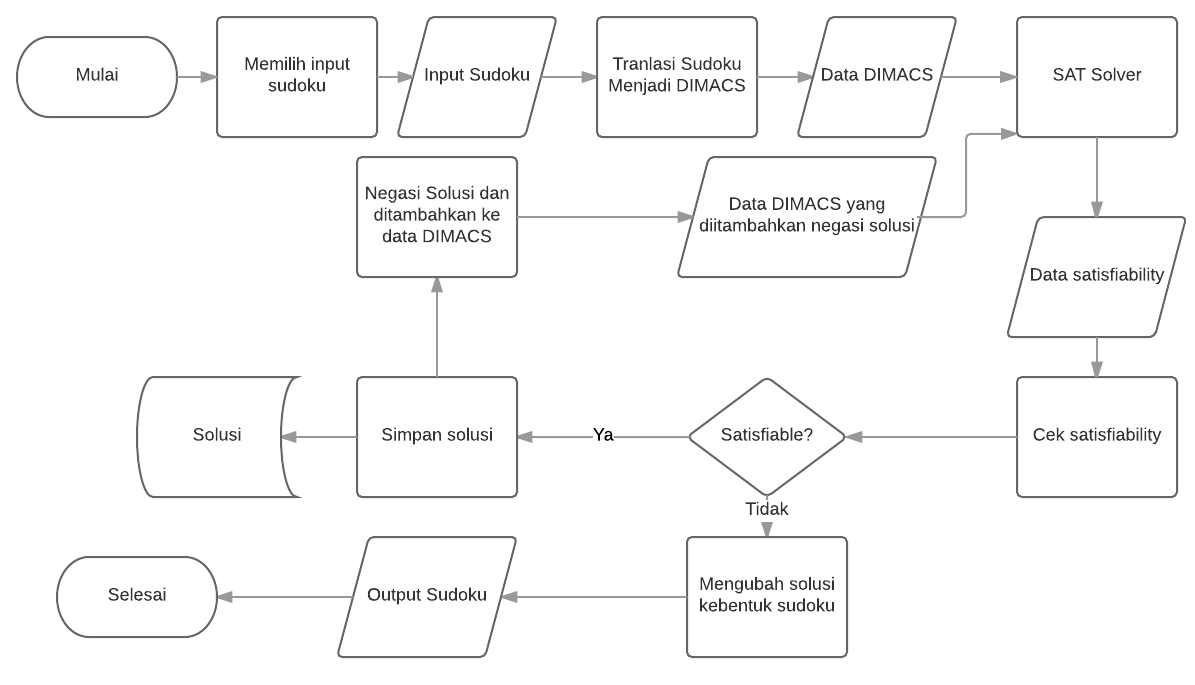
\includegraphics[scale=0.5]{gambar/diagramAlir.png}
		
		\caption{Diagram alir.}
	\end{centering}
\end{figure}

\section{Pembuatan aplikasi}

Pembuatan aplikasi pemecah sudoku interaktif berbasis Python.

\subsection{Use Case}

\begin{figure}[H]
	\begin{centering}
		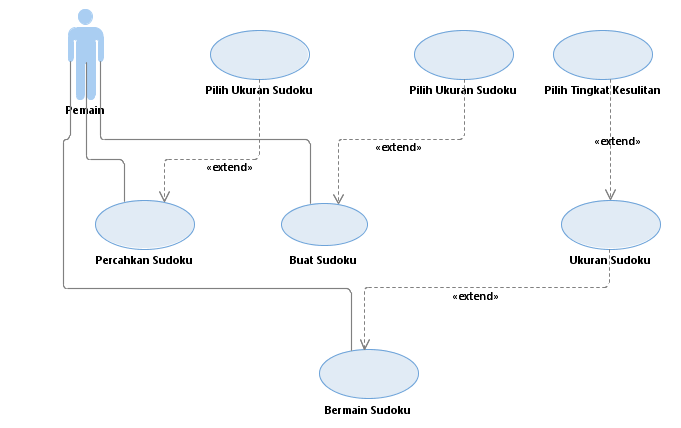
\includegraphics[scale=1]{gambar/useCase}
		
		\caption{\textit{Use Case Diagram}.}
	\end{centering}
\end{figure}

Fungsionalitas aplikasi adalah sebagai berikut:
\begin{enumerate}
	\item Bermain sudoku.
	\item Membuat sudoku.
	\item Memecahkan sudoku.
	\item Pilih ukuran sudoku.
	\item Pilih kesulitan sudoku.
\end{enumerate}

\subsection{Aturan Sudoku Dalam Python}

Aturan-aturan yang ada dalam bentuk CNF di ubah kedalam bahasa Python serta dibuatkan aturan DIMACSnya.

\begin{enumerate}
	\item Setiap baris memuat bilangan antara 1 
	hingga 9 : 
	
	$\bigwedge_{r=1}^{9}$$\bigwedge_{n=1}^{9}$$\bigvee_{c=1}^{9}$$p\left(r,c,n\right)$
	
	\vspace{5mm}
	
	Skrip Python :
	
	\vspace{5mm}
	
	\texttt{def aturan1(dimacs):}
	
	\quad\quad\texttt{for r in range(1, 10):}
	
	\quad\quad\quad\texttt{for n in range(1, 10):}
	
	\quad\quad\quad\quad\texttt{for c in range(1, 10):}
	
	\quad\quad\quad\quad\quad\texttt{dimacs += str(r) + str(c) + str(n) + ' '}
	
	\quad\quad\quad\quad\texttt{dimacs += '0\textbackslash n'}
	
	\quad\quad\quad\quad\texttt{klausa += 1}
	
	\quad\quad\texttt{return dimacs}
	
	
	\item Setiap kolom memuat bilangan antara 1 hingga 9 : 
	
	$\bigwedge_{c=1}^{9}$$\bigwedge_{n=1}^{9}$$\bigvee_{r=1}^{9}$$p\left(r,c,n\right)$
	
	
	\vspace{5mm}
	
	Skrip Python :
	
	\vspace{5mm}
	
	\texttt{def aturan2(dimacs):}
	
	\quad \quad\texttt{for c in range(1, 10):}
	
	\quad \quad \quad\texttt{for n in range(1, 10):}
	
	\quad \quad \quad \quad\texttt{for r in range(1, 10):}
	
	\quad\quad\quad\quad\quad\texttt{dimacs += str(r) + str(c) + str(n) + ' '}
	
	\quad \quad \quad \quad\texttt{dimacs += '0\textbackslash n'}
	
	\quad \quad \quad \quad\texttt{klausa += 1}
	
	\quad \quad\texttt{return dimacs}
	
	\item Setiap submatriks atau blok $3 \times 3$
	memuat bilangan antara 1 hingga 9 : 
	
	$\bigwedge_{i=0}^{2}$$\bigwedge_{j=0}^{2}$$\bigwedge_{n=1}^{9}$$\bigvee_{r=3i+1}^{3i+3}$$\bigvee_{c=3j+1}^{3j+3}$$p\left(r,c,n\right)$
	
	
	\vspace{5mm}
	
	Skrip Python :
	
	\vspace{5mm}
	
	\texttt{def aturan3(dimacs):}
	
	\quad \quad\texttt{for i in range(0, 3):}
	
	\quad \quad \quad\texttt{for j in range(0, 3):}
	
	\quad \quad \quad \quad\texttt{for n in range(1, 10):}
	
	\quad\quad\quad\quad\quad\texttt{for r in range(3*i+1, 3*i+4):}
	
	\quad\quad\quad\quad\quad\quad\texttt{for c in range(3*j+1, 3*j+4):}
	
	\quad\quad\quad\quad\quad\quad\quad\texttt{dimacs += str(r) + str(c) + str(n) + ' '}
	
	\quad\quad\quad\quad\quad\texttt{dimacs += '0\textbackslash n'}
	
	\quad\quad\quad\quad\quad\texttt{klausa += 1}
	
	\quad\quad\texttt{return dimacs}
	
	\vspace{5mm}
	
	
	\item Setiap sel memuat paling banyak satu bilangan antara 1 hingga 9 : 
	
	$\bigwedge_{r=1}^{9}$$\bigwedge_{c=1}^{9}$$\bigwedge_{n=1}^{8}$$\bigwedge_{i=n+1}^{9}$
	$\left(\neg p\left(r,c,n\right)\vee\neg p\left(r,c,i\right)\right)$
	
	
	\vspace{5mm}
	
	Skrip Python :
	
	\vspace{5mm}
	
	\texttt{def aturan4(dimacs):}
	
	\quad \quad\texttt{for e in range(0, 3):}
	
	\quad \quad \quad\texttt{for c in range(0, 3):}
	
	\quad \quad \quad \quad\texttt{for n in range(1, 9):}
	
	\quad\quad\quad\quad\quad\texttt{for i in range(n+1, 10):}
	
	\quad\quad\quad\quad\quad\quad\texttt{dimacs += '-' + str(r) + str(c) + str(n) + ' ' + '-'} 
	
	\quad\quad\quad\quad\quad\quad\texttt{+ str(r) + str(c) + str(i) + ' 0\textbackslash n'}
	
	\quad\quad\quad\quad\quad\texttt{klausa += 1}
	
	\quad \quad\texttt{return dimacs}
	
\end{enumerate}

\section{Pengujian aplikasi}

Pada tahap ini aplikasi akan diujikan kebeberapa penguji dengan diberikan lembar \textit{test plan} yang meliputi beberapa aspek kualitas pada aplikasi. Teknik yang digunakan pada pengujian adalah pengujian kotak hitam \cite{TEST1}.

\section{Analisis aplikasi}

Menganalisa kesusaian keluaran dari aplikasi berdasarkan hasil dari pengujian.